\chapter{Processes}

\section{Chapter Overview}

Processes are among the most frequently tested operating system topics in Software Development Engineer interviews. Companies such as Amazon, Google, Microsoft, Meta, Uber, Atlassian, Bloomberg, and Apple expect candidates to understand process creation, process management, context switching, scheduling, and Linux process internals.

This chapter builds a strong conceptual and interview-oriented understanding of processes.

\section{Learning Objectives}

After completing this chapter, you should be able to:

\begin{itemize}
\item Define a process and explain its characteristics.
\item Differentiate between a program and a process.
\item Understand process memory layout.
\item Explain process states and state transitions.
\item Describe the Process Control Block (PCB).
\item Understand context switching.
\item Explain process creation and termination.
\item Understand fork(), exec(), and wait().
\item Identify zombie and orphan processes.
\item Understand daemon processes.
\item Explain Linux process management.
\end{itemize}

%--------------------------------------------------
\section{Process Concept}
%--------------------------------------------------

\subsection{Definition}

A \textbf{process} is a program in execution.

A process consists of:

\begin{itemize}
\item Program code
\item Program counter
\item CPU registers
\item Stack
\item Heap
\item Open files
\item Process state
\end{itemize}

\subsection{Real-World Analogy}

Consider a recipe and a chef.

\begin{itemize}
\item Recipe = Program
\item Chef executing recipe = Process
\end{itemize}

Multiple chefs can execute the same recipe simultaneously.

Similarly, multiple processes can execute the same program.

\subsection{Examples}

\begin{itemize}
\item Google Chrome
\item VS Code
\item MySQL Server
\item Python Interpreter
\end{itemize}

Each running instance is a process.

%--------------------------------------------------
\section{Program vs Process}
%--------------------------------------------------

\begin{table}[H]
\centering
\begin{tabular}{|p{4cm}|p{5.5cm}|p{5.5cm}|}
\hline
Feature & Program & Process \\
\hline
Definition & Passive entity & Active entity \\
\hline
Stored On & Disk & Memory \\
\hline
Execution & Not executing & Executing \\
\hline
State & Static & Dynamic \\
\hline
Resources & No resources allocated & Resources allocated \\
\hline
Example & chrome.exe & Running Chrome instance \\
\hline
\end{tabular}
\caption{Program vs Process}
\end{table}

\subsection{Interview Tip}

A program becomes a process when loaded into memory and executed by the CPU.

%--------------------------------------------------
\section{Process Memory Layout}
%--------------------------------------------------

Every process has its own virtual address space.

\begin{figure}[H]
\centering
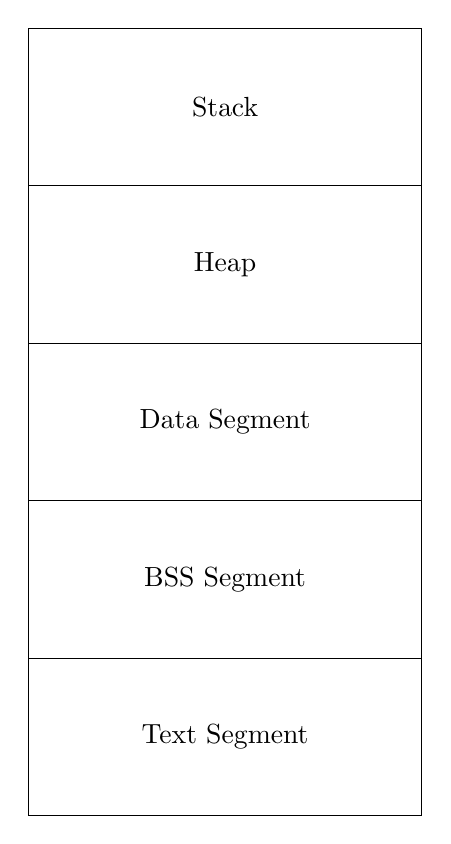
\begin{tikzpicture}

\draw (0,0) rectangle (5,10);

\draw (0,8) -- (5,8);
\draw (0,6) -- (5,6);
\draw (0,4) -- (5,4);
\draw (0,2) -- (5,2);

\node at (2.5,9) {Stack};
\node at (2.5,7) {Heap};
\node at (2.5,5) {Data Segment};
\node at (2.5,3) {BSS Segment};
\node at (2.5,1) {Text Segment};

\end{tikzpicture}
\caption{Typical Process Memory Layout}
\end{figure}

\subsection{Text Segment}

Contains executable instructions.

\subsection{Data Segment}

Stores initialized global and static variables.

\subsection{BSS Segment}

Stores uninitialized global and static variables.

\subsection{Heap}

Used for dynamic memory allocation.

Examples:

\begin{verbatim}
malloc()
calloc()
new
\end{verbatim}

\subsection{Stack}

Stores:

\begin{itemize}
\item Function calls
\item Local variables
\item Return addresses
\end{itemize}

\subsection{Interview Question}

\textbf{Stack grows in which direction?}

Typically toward lower memory addresses.

\textbf{Heap grows in which direction?}

Typically toward higher memory addresses.

%--------------------------------------------------
\section{Process States}
%--------------------------------------------------

\subsection{Five-State Model}

\begin{enumerate}
\item New
\item Ready
\item Running
\item Waiting (Blocked)
\item Terminated
\end{enumerate}

\begin{figure}[H]
\centering
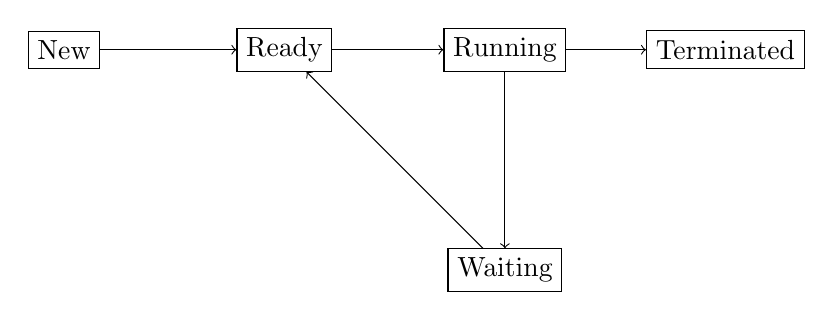
\begin{tikzpicture}[node distance=2.8cm]

\node[draw] (new) {New};
\node[draw,right of=new] (ready) {Ready};
\node[draw,right of=ready] (running) {Running};
\node[draw,below of=running] (waiting) {Waiting};
\node[draw,right of=running] (terminated) {Terminated};

\draw[->] (new) -- (ready);
\draw[->] (ready) -- (running);
\draw[->] (running) -- (waiting);
\draw[->] (waiting) -- (ready);
\draw[->] (running) -- (terminated);

\end{tikzpicture}
\caption{Process State Transition Diagram}
\end{figure}

\subsection{Ready State}

Waiting for CPU.

\subsection{Running State}

Currently executing.

\subsection{Waiting State}

Waiting for an event or I/O completion.

\subsection{Terminated State}

Execution completed.

%--------------------------------------------------
\section{Process Control Block (PCB)}
%--------------------------------------------------

\subsection{Definition}

PCB is a kernel data structure containing information about a process.

\subsection{Contents of PCB}

\begin{itemize}
\item Process ID (PID)
\item Process State
\item Program Counter
\item CPU Registers
\item Scheduling Information
\item Memory Information
\item Open Files
\item Accounting Information
\end{itemize}

\begin{figure}[H]
\centering
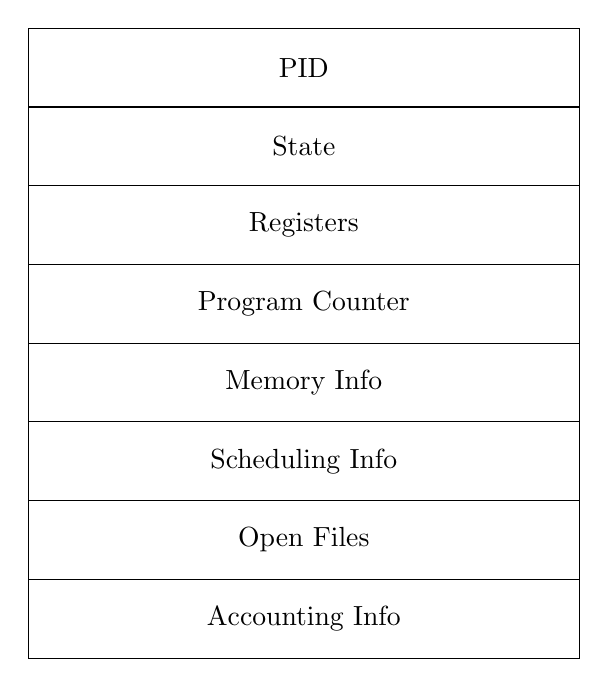
\begin{tikzpicture}

\draw (0,0) rectangle (7,8);

\draw (0,7) -- (7,7);
\draw (0,6) -- (7,6);
\draw (0,5) -- (7,5);
\draw (0,4) -- (7,4);
\draw (0,3) -- (7,3);
\draw (0,2) -- (7,2);
\draw (0,1) -- (7,1);

\node at (3.5,7.5) {PID};
\node at (3.5,6.5) {State};
\node at (3.5,5.5) {Registers};
\node at (3.5,4.5) {Program Counter};
\node at (3.5,3.5) {Memory Info};
\node at (3.5,2.5) {Scheduling Info};
\node at (3.5,1.5) {Open Files};
\node at (3.5,0.5) {Accounting Info};

\end{tikzpicture}
\caption{Process Control Block}
\end{figure}

%--------------------------------------------------
\section{Context Switching}
%--------------------------------------------------

\subsection{Definition}

Context switching is the process of saving the state of one process and loading the state of another.

\subsection{Steps}

\begin{enumerate}
\item Save current process context into PCB.
\item Select next process.
\item Load next process context.
\item Resume execution.
\end{enumerate}

\begin{figure}[H]
\centering
\begin{tikzpicture}

\node[draw] (p1) {Process A};
\node[draw,right=4cm of p1] (p2) {Process B};

\draw[->] (p1) -- node[above]{Save Context} (p2);
\draw[->] (p2) -- node[below]{Load Context} (p1);

\end{tikzpicture}
\caption{Context Switch}
\end{figure}

\subsection{Interview Insight}

Context switching is pure overhead because no useful work is performed during the switch.

%--------------------------------------------------
\section{Process Creation}
%--------------------------------------------------

Most operating systems allow processes to create child processes.

\subsection{Linux Model}

Parent process creates child process using:

\begin{verbatim}
fork()
\end{verbatim}

\subsection{Windows Model}

Uses:

\begin{verbatim}
CreateProcess()
\end{verbatim}

%--------------------------------------------------
\section{fork()}
%--------------------------------------------------

\subsection{Definition}

fork() creates a new process by duplicating the calling process.

\subsection{Return Values}

\begin{table}[H]
\centering
\begin{tabular}{|c|c|}
\hline
Return Value & Meaning \\
\hline
0 & Child Process \\
\hline
$>$0 & Parent Process \\
\hline
-1 & Error \\
\hline
\end{tabular}
\caption{fork() Return Values}
\end{table}

\subsection{Example}

\begin{lstlisting}[language=C]
#include <stdio.h>
#include <unistd.h>

int main()
{
    pid_t pid = fork();

    if(pid == 0)
        printf("Child Process\n");
    else
        printf("Parent Process\n");

    return 0;
}
\end{lstlisting}

\subsection{Interview Insight}

After fork():

\begin{itemize}
\item Parent and child have separate address spaces.
\item Modern systems use Copy-On-Write (COW).
\end{itemize}

%--------------------------------------------------
\section{exec()}
%--------------------------------------------------

\subsection{Definition}

exec() replaces the current process image with a new program.

\subsection{Common Variants}

\begin{itemize}
\item execl()
\item execlp()
\item execv()
\item execvp()
\end{itemize}

\subsection{Example}

\begin{lstlisting}[language=C]
#include <unistd.h>

int main()
{
    execl("/bin/ls","ls","-l",NULL);
    return 0;
}
\end{lstlisting}

\subsection{Important Point}

exec() does not create a new process.

It replaces the current process image.

%--------------------------------------------------
\section{wait()}
%--------------------------------------------------

\subsection{Definition}

wait() causes the parent process to wait for child termination.

\subsection{Example}

\begin{lstlisting}[language=C]
#include <sys/wait.h>
#include <unistd.h>

int main()
{
    if(fork()==0)
        return 0;

    wait(NULL);
}
\end{lstlisting}

\subsection{Purpose}

Prevents zombie processes.

%--------------------------------------------------
\section{Process Scheduling Overview}
%--------------------------------------------------

The scheduler selects a process from the ready queue.

Goals:

\begin{itemize}
\item High CPU utilization
\item Fairness
\item Low response time
\item High throughput
\end{itemize}

Common scheduling algorithms:

\begin{itemize}
\item FCFS
\item SJF
\item Priority Scheduling
\item Round Robin
\item Multilevel Queue
\end{itemize}

%--------------------------------------------------
\section{Process Termination}
%--------------------------------------------------

A process may terminate due to:

\begin{itemize}
\item Normal completion
\item Error
\item Fatal exception
\item Parent termination
\item Explicit kill signal
\end{itemize}

Linux commands:

\begin{verbatim}
kill PID
kill -9 PID
pkill process_name
\end{verbatim}

%--------------------------------------------------
\section{Zombie Processes}
%--------------------------------------------------

\subsection{Definition}

A zombie process is a terminated process whose PCB still exists.

\subsection{Reason}

Parent has not collected exit status.

\subsection{Characteristics}

\begin{itemize}
\item Process finished execution.
\item Entry remains in process table.
\item Consumes PID slot.
\end{itemize}

\subsection{Fix}

Parent must call:

\begin{verbatim}
wait()
waitpid()
\end{verbatim}

\subsection{Linux Example}

\begin{verbatim}
ps aux | grep Z
\end{verbatim}

%--------------------------------------------------
\section{Orphan Processes}
%--------------------------------------------------

\subsection{Definition}

An orphan process is a child process whose parent terminates before it.

\subsection{What Happens?}

The orphan is adopted by:

\begin{verbatim}
init (PID 1)
\end{verbatim}

or

\begin{verbatim}
systemd
\end{verbatim}

\subsection{Interview Question}

\textbf{Zombie vs Orphan?}

Zombie:
Parent alive, child terminated.

Orphan:
Parent terminated, child alive.

%--------------------------------------------------
\section{Daemon Processes}
%--------------------------------------------------

\subsection{Definition}

A daemon is a background process providing system services.

\subsection{Characteristics}

\begin{itemize}
\item No terminal
\item Long-running
\item Starts during boot
\end{itemize}

Examples:

\begin{itemize}
\item sshd
\item cron
\item systemd
\item httpd
\end{itemize}

Linux command:

\begin{verbatim}
ps -ef
\end{verbatim}

%--------------------------------------------------
\section{Process Hierarchies}
%--------------------------------------------------

Processes form a tree structure.

\begin{figure}[H]
\centering
\begin{tikzpicture}

\node[draw] (init) {init/systemd};

\node[draw,below left=1.5cm and 2cm of init] (bash) {bash};
\node[draw,below right=1.5cm and 2cm of init] (sshd) {sshd};

\node[draw,below=1.5cm of bash] (vim) {vim};

\draw (init)--(bash);
\draw (init)--(sshd);
\draw (bash)--(vim);

\end{tikzpicture}
\caption{Process Hierarchy}
\end{figure}

%--------------------------------------------------
\section{Linux Process Management}
%--------------------------------------------------

\subsection{Useful Commands}

\begin{table}[H]
\centering
\begin{tabular}{|p{4cm}|p{8cm}|}
\hline
Command & Purpose \\
\hline
ps & Display processes \\
\hline
top & Process monitoring \\
\hline
htop & Interactive monitoring \\
\hline
pstree & Process tree \\
\hline
kill & Terminate process \\
\hline
nice & Set priority \\
\hline
renice & Modify priority \\
\hline
\end{tabular}
\caption{Linux Process Commands}
\end{table}

\subsection{Examples}

View process tree:

\begin{verbatim}
pstree
\end{verbatim}

Monitor processes:

\begin{verbatim}
top
\end{verbatim}

Kill process:

\begin{verbatim}
kill -9 1234
\end{verbatim}

%--------------------------------------------------
\section{Interview Insights}
%--------------------------------------------------

Frequently asked topics:

\begin{itemize}
\item fork() vs exec()
\item Zombie vs Orphan
\item PCB contents
\item Context switching overhead
\item Copy-On-Write
\item Process states
\item Linux process commands
\item Process hierarchy
\end{itemize}

\textbf{Golden Rule:}

If asked about process creation in Linux:

\begin{center}
fork() $\rightarrow$ exec() $\rightarrow$ wait()
\end{center}

%--------------------------------------------------
\section{Key Takeaways}
%--------------------------------------------------

\begin{itemize}
\item Process is a program in execution.
\item PCB stores process information.
\item Context switching saves and restores process state.
\item fork() creates a child process.
\item exec() replaces process image.
\item wait() synchronizes parent and child.
\item Zombies are terminated processes awaiting cleanup.
\item Orphans are adopted by init/systemd.
\item Daemons provide background services.
\item Linux provides powerful process management tools.
\end{itemize}

%--------------------------------------------------
\section{20 Interview Questions with Answers}
%--------------------------------------------------

\begin{enumerate}
\item What is a process?\\
Answer: Program in execution.

\item Program vs Process?\\
Answer: Program is passive; process is active.

\item What is PCB?\\
Answer: Kernel data structure storing process information.

\item What is PID?\\
Answer: Process Identifier.

\item What is context switching?\\
Answer: Saving one process state and restoring another.

\item Why is context switching expensive?\\
Answer: It performs no useful work.

\item What does fork() do?\\
Answer: Creates a child process.

\item fork() return value in child?\\
Answer: 0.

\item fork() return value in parent?\\
Answer: Child PID.

\item What does exec() do?\\
Answer: Replaces process image.

\item Does exec() create a process?\\
Answer: No.

\item Purpose of wait()?\\
Answer: Waits for child termination.

\item What is a zombie process?\\
Answer: Terminated process awaiting cleanup.

\item What is an orphan process?\\
Answer: Child whose parent terminated.

\item Who adopts orphan processes?\\
Answer: init/systemd.

\item What is a daemon?\\
Answer: Background service process.

\item What is Copy-On-Write?\\
Answer: Memory copied only upon modification.

\item What is process scheduling?\\
Answer: Selecting next process for CPU.

\item What is a ready queue?\\
Answer: Queue of runnable processes.

\item What Linux command shows processes?\\
Answer: ps.
\end{enumerate}

%--------------------------------------------------
\section{20 MCQs with Answers}
%--------------------------------------------------

\begin{enumerate}
\item Process is:
A) Hardware
B) Program in execution
C) Compiler
D) Kernel

Answer: B

\item PCB stands for:
Answer: Process Control Block

\item fork() creates:
Answer: Child Process

\item exec() creates a new process.
Answer: False

\item wait() prevents:
Answer: Zombie Processes

\item Process state waiting means:
Answer: Waiting for event/I/O

\item Linux process ID is:
Answer: PID

\item Stack stores:
Answer: Function calls

\item Heap stores:
Answer: Dynamic allocations

\item Zombie process is:
Answer: Terminated but not reaped

\item Orphan process is:
Answer: Parent terminated

\item Daemon process runs:
Answer: Background

\item Scheduler selects from:
Answer: Ready Queue

\item Context switch stores:
Answer: CPU State

\item Linux tree command:
Answer: pstree

\item kill -9 sends:
Answer: SIGKILL

\item Child PID returned to:
Answer: Parent

\item Program becomes process when:
Answer: Executed

\item Copy-On-Write improves:
Answer: Efficiency

\item Running process uses:
Answer: CPU
\end{enumerate}

%--------------------------------------------------
\section{Revision Notes}
%--------------------------------------------------

\begin{itemize}
\item Process = Program + Execution State.
\item PCB stores process metadata.
\item fork() duplicates process.
\item exec() replaces process image.
\item wait() synchronizes parent and child.
\item Context switching causes overhead.
\item Zombie = dead child not reaped.
\item Orphan = living child without parent.
\item Daemon = background service.
\item Linux process tree begins at init/systemd.
\end{itemize}

%--------------------------------------------------
\section{Cheat Sheet}
%--------------------------------------------------

\begin{center}
\begin{tabular}{|p{5cm}|p{8cm}|}
\hline
Process & Program in execution \\
\hline
PCB & Process metadata \\
\hline
fork() & Create child process \\
\hline
exec() & Replace process image \\
\hline
wait() & Wait for child \\
\hline
PID & Process identifier \\
\hline
Zombie & Dead child not cleaned \\
\hline
Orphan & Child without parent \\
\hline
Daemon & Background process \\
\hline
Ready State & Waiting for CPU \\
\hline
Running State & Using CPU \\
\hline
Waiting State & Waiting for event \\
\hline
Context Switch & Save + Restore CPU state \\
\hline
pstree & Show hierarchy \\
\hline
top & Monitor processes \\
\hline
kill -9 & Force termination \\
\hline
\end{tabular}
\end{center}